\documentclass{standalone}
\usepackage{tikz}
\usetikzlibrary{calc,patterns,decorations.pathmorphing,decorations.markings}

\begin{document}

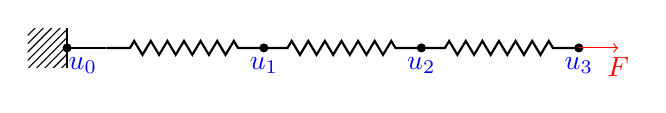
\begin{tikzpicture}[every node/.style={outer sep=0pt,thick}]
\tikzset{
    spring/.style = {thick,decorate,decoration={zigzag,pre length=0.3cm,post length=0.3cm,segment 
                        length=6}},
    damper/.style ={thick,decoration={markings,
                        mark connection node=dmp,
                        mark=at position 0.5 with
                            {
                            \node (dmp) [thick,inner sep=0pt,transform shape,rotate=-90,minimum 
                                    width=15pt,minimum height=3pt,draw=none] {};
                            \draw [thick] ($(dmp.north east)+(1pt,0)$) -- (dmp.south east) -- (dmp.south 
                                    west) -- ($(dmp.north west)+(1pt,0)$);
                            \draw [thick] ($(dmp.north)+(0,-5pt)$) -- ($(dmp.north)+(0,5pt)$);
                            }
                        }, decorate},
    ground/.style ={fill,pattern=north east lines,draw=none,minimum width=0.5cm,minimum height=0.5cm}
}

\begin{scope}[rotate=-90,transform shape]       %%% rotate here, both options needed.

\node (wall) [ground,anchor=center] at (0,0) {};

\draw (wall.north east) -- (wall.north west);


%% now a parallel spring
\draw [line width=0.8pt] ($(wall.north west)!0.5!(wall.north east)$) -- ++(0,0.5cm)coordinate (z);
\draw[black,fill=black] ($(wall.north west)!0.5!(wall.north east)$) circle (0.05);
\draw  ($(wall.north west)!0.5!(wall.north east)$)+(0,0.2cm) node[below, rotate=+90, blue] {$u_0$}; 
\draw [spring] (z) -- ++(0,2cm)coordinate (t1);
\draw[black, fill=black] (t1) circle (0.05) ; 
\draw (t1) node[below, rotate=+90, blue] {$u_1$}; 
\draw [spring] (t1) -- ++(0,2cm)coordinate (t2);
\draw[black, fill=black] (t2) circle (0.05) ; 
\draw (t2) node[below, rotate=+90, blue] {$u_2$}; 
\draw [spring] (t2) -- ++(0,2cm)coordinate (t3);
\draw[black, fill=black] (t3) circle (0.05) ;
\draw (t3) node[below, rotate=+90, blue] {$u_3$}; 
\draw[->, red] (t3) -- ++(0,0.5cm)coordinate(f);
\draw (f) node[below, rotate=+90, red] {$F$}; 

%%%\draw [line width=0.8pt] (t) -- ($(walle.south west)!0.2!(walle.south east)$);

\end{scope}


%%\begin{scope}[rotate=-90,transform shape]       %%% rotate here, both options needed.

%%\draw [line width=0.8pt] ($(wall.north west)!0.8!(wall.north east)$) -- ++(0,1cm)coordinate (z);
%%\draw [spring] (z) -- ++(0,2cm)coordinate (t); 
%%\draw [damper] (t) -- ++(0,2cm)coordinate (u); 
%%\draw [line width=0.8pt] (u) -- ($(walle.south west)!0.8!(walle.south east)$);

%%\end{scope}

\end{tikzpicture}

\end{document}
